%%%%%%%%%%%%%%%%%%%%%%% file template.tex %%%%%%%%%%%%%%%%%%%%%%%%%
%
% This is a general template file for the LaTeX package SVJour3
% for Springer journals.          Springer Heidelberg 2010/09/16
%
% Copy it to a new file with a new name and use it as the basis
% for your article. Delete % signs as needed.
%
% This template includes a few options for different layouts and
% content for various journals. Please consult a previous issue of
% your journal as needed.
% 
%%%%%%%%%%%%%%%%%%%%%%%%%%%%%%%%%%%%%%%%%%%%%%%%%%%%%%%%%%%%%%%%%%%
%
% First comes an example EPS file -- just ignore it and
% proceed on the \documentclass line
% your LaTeX will extract the file if required
\begin{filecontents*}{example.eps}
%!PS-Adobe-3.0 EPSF-3.0
%%BoundingBox: 19 19 221 221
%%CreationDate: Mon Sep 29 1997
%%Creator: programmed by hand (JK)
%%EndComments
gsave
newpath
  20 20 moveto
  20 220 lineto
  220 220 lineto
  220 20 lineto
closepath
2 setlinewidth
gsave
  .4 setgray fill
grestore
stroke
grestore
\end{filecontents*}
%
\RequirePackage{fix-cm}
%
%\documentclass{svjour3}                     % onecolumn (standard format)
%\documentclass[smallcondensed]{svjour3}     % onecolumn (ditto)
\documentclass[smallextended]{svjour3}       % onecolumn (second format)
%\documentclass[twocolumn]{svjour3}          % twocolumn
%
\smartqed  % flush right qed marks, e.g. at end of proof
%
\usepackage{graphicx}
\usepackage{amsmath}
\usepackage{amssymb}
\usepackage{soul}
\usepackage{multicol}

\newcommand{\hilight}[1]{\hl{#1}}
 
\newcommand{\mynote}[2]{
    {\bfseries\sffamily\scriptsize\hilight{#1}}
    {\small$\blacktriangleright$\hilight{#2}$\blacktriangleleft$}}
\newcommand\todo[1]{\mynote{TODO}{#1}} 
\newcommand{\fig}[1]{Fig.\;\ref{#1}}
\newcommand{\sect}[1]{Section\;\ref{#1}}


\newcommand{\ct}[1]{\textit{{#1}}}

\usepackage{verbatim}
\newenvironment{code}
	{\footnotesize \verbatim}
	{\endverbatim \normalsize}

\usepackage{listings}

\newcommand{\phead}[1]{\vspace{8pt}\noindent$\blacksquare$\hspace{3pt}\textit{{#1}.}\hspace{8pt}}

%
% \usepackage{mathptmx}      % use Times fonts if available on your TeX system
%
% insert here the call for the packages your document requires
%\usepackage{latexsym}
% etc.
%
% please place your own definitions here and don't use \def but
% \newcommand{}{}
%
% Insert the name of "your journal" with
% \journalname{myjournal}
%
\begin{document}

\title{Language and IDE Modularization, Extension and Composition with MPS}

%\titlerunning{Short form of title}        % if too long for running head

\author{Markus Voelter}

%\authorrunning{Short form of author list} % if too long for running head

\institute{Markus Voelter \at
              Oetztaler Strasse 38, Stuttgart, Germany \\
              \email{voelter@acm.org}           %  \\
}

\date{Received: date / Accepted: date}
% The correct dates will be entered by the editor


\maketitle

\begin{abstract}
Language modularization, extension and composition is an important building
block for working efficiently with DSLs. Historically, this has been a challenge
because many grammar formalisms are not closed under composition, hence
syntactic composition of languages is challenging. Composing static and dynamic
semantics can also be hard, at least in the general case. Finally, a lot of
existing work does not consider IDEs for the composed and extended languages. In
this paper, I will show how the projectional language workbench JetBrains MPS
solves most of these issues in a practically usable way. The main part of the
paper is an extensive example that shows the various kinds of extension and
modularization. The last section contains an evaluation that identifies the
strong and weak aspects of modularization, composition and extension in MPS, and
suggests a couple of improvements.
\keywords{DSLs \and language composition \and language extension \and JetBrains
MPS \and Language Workbench}
% \PACS{PACS code1 \and PACS code2 \and more}
% \subclass{MSC code1 \and MSC code2 \and more}
\end{abstract}



\section{Introduction}
\label{intro}

\subsection{Approach and Structure of the paper}

Language modularization, extension and composition (LME\&C) is an important
ingredient to the efficient use of DSLs, just like reuse in general is important
to software development. We discuss the need for LME\&C in the context of DSL
design in \cite{VoelterVisserDimensions2011}, where we also introduce some of the
terminology used in this paper. Traditionally, LME\&C, including the respective
IDEs, has been hard for various reasons, including limited composability of
grammars, non-modular IDEs as well as semantic interactions. Specifically,
LME\&C, requires the following concerns to be considered:


\begin{itemize}
  \item The concrete and the abstract syntax have to be combined. Depending on
  the kind of composition, this requires the embedding of one syntax into
  another one. This, in turn, requires modular grammars.
  \item The static semantics, i.e. the constraints and the type system have to
  be integrated. For example in case of language extension, new types have to be
  "made valid" for existing operators.
  \item The execution semantics have to be combined as well. In practice, this
  may mean mixing the code generated from the composed languages, or composing
  the generators.
  \item Finally, the IDE that provides code completion, syntax coloring, static
  checks and other relevant services has to be extended and composed as well.
\end{itemize}

With JetBrains MPS two of these challenges --- composability of concrete syntax
and modular IDEs --- are a completely solved problem, as this paper will show.
Modular type systems are reasonably well supported. Semantic interactions are
hard to solve in general, but can be handled reasonably in many relevant cases,
as we show in this paper as well. However, as we will see, in many cases,
languages have to be designed \emph{explicitly for reuse}, in order to make them
reusable. After-the-fact reuse, without considering it during the design of the
reusable language, is possible only in limited cases. However, this is true for
reuse in software generally.

The paper is structured as follows. In \sect{typesOfMod} we outline the various
kinds of LME\&C as defined and explained in the \cite{VoelterVisserDimensions2011} paper.
Then we describe how projectional editors work in general, and how MPS works specifically
(\sect{HowMPSWorks}). Next we provide a brief overview over related tools and
approaches to illustrate how MPS is different (\sect{Related}). Then we develop
the core language which acts as the basis for the extension and composition
examples. We use the simplest possible language, entities, for this task. This
section (\sect{entitiesLanguage}) also serves as a very brief tutorial on
language definition in MPS. The main part of the paper, the implementation of
the various extension and composition approaches is discussed in
\sect{extAndComp}. Finally, \sect{Eval} looks at what works well and at what
could be improved in MPS with regards to extension and composition.


\subsection{Additional Resources}

The example code developed for this tutorial can be found at github.com:

\vspace{5pt}
\verb#https://github.com/markusvoelter/MPS-Language-Composition-Demos---For-MPS-2.0#
\vspace{5pt}

\noindent It is developed with MPS 2.0 M6 and should run with the final version
of MPS 2.0 as well. At the point of this writing, MPS 2.0 had not yet been released and
hence I couldn't test it.

A set of recorded demos (90 minutes in total) that walk through all the example
code is available on Youtube. The initial video is here: 

\vspace{5pt}
\verb#http://www.youtube.com/watch?v=lNMRMZk8KBE#. 
\vspace{5pt}

\noindent The others are either suggested by Youtube, or you can find them by
searching for \emph{Language Modularization and Composition with MPS (Part X)}, where X is
between 1 and 8.

Note that this paper cannot be a complete MPS tutorial. MPS is very deep and
powerful, so we have to focus on those aspects that are essential for LME\&C. We
refer to the LWC 11 MPS tutorial for a at detailed MPS tutorial:

\vspace{5pt}
\verb+http://code.google.com/p/mps-lwc11/wiki/GettingStarted+


\subsection{Types of Modularization}
\label{typesOfMod}


As we describe in the paper on DSL design dimensions
\cite{VoelterVisserDimensions2011}, we distinguish language \emph{combination}, \emph{extension}, \emph{reuse} and
\emph{embedding}.


\phead{Extension} A language B extends another language A if B contains
additional language concepts. This means that for programs written in B, all
concepts from A are available, plus those defined in B. Concepts in B may
specialize concepts in A. This means that in B programs, the specialized concept
can be used wherever A programs expect only the more general one, effectively
adapting the Liskov substitution principle to language concepts. An extended
language may also restrict the base language, so certain concepts are not
available in the sublanguge.


\phead{Combination} If a domain is structured along different concerns, and
these concerns should be implemented using separate viewpoints, then it is often
useful to implement every concern as a separate DSL. When these DSL are
developed from scratch, as a group, then dependencies between the concerns can
be materialized as dependencies between the languages and the language concepts.
A language B may depend on language A because a concept in language B references
a concept in language A. The models remain separate, only cross-references
connect the two.
 
\phead{Reuse} Reuse describes the case where a language has been developed
explicitly to be used in contexts not known at the time of development of that
language (this is in contrast to combination). So the language cannot have
dependencies to other languages. To make it fit in with a new context, the
reusable language has to be extended so it can reference concepts from languages
in that context.


\phead{Embedding} Embedding is a special case of reuse, where the reused
language is syntactically embedded into languages from the context. If the host
language is designed with an awareness of the composed language, the host
language can simply depend on the composed language and embed concepts from it.
As in the case of language reuse, the composed language may have to be extended
to "plug it into the context". If both the host language and the composed
language have been designed independent of each other and should be combined
later, then both the host language and the composed language will have to be
extended.

\vspace{8pt}
In this paper we illustrate all of these approaches with MPS. At the center is a
simple entities language. We then build additional language to illustrate
LME\&C. \fig{languagestructure} illustrates these additional languages. The
uispec language illustrates \emph{combination} with entities. relmapping is an
example of \emph{reuse} with separated generated code. \emph{rbac} illustrates
reuse with intermixed generated code. uispec\_validation demonstrates
\emph{extension} (of the uispec language) and \emph{embedding} with regards to
the expressions language.


\begin{figure}[htp]
\begin{center}
  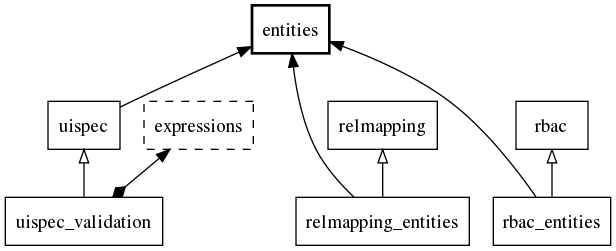
\includegraphics[scale=0.4]{figures/languagestructure.png}
  \caption[labelInTOC]{entities is the central language. uispec defines UI
  forms for the entities. uispec\_validation adds validation rules, and composes
  a reusable expressions language. relmapping provides a reusable database
  mapping language, relmapping\_entities adapts it to the entities language.
  rbac is a reusable language for specifying permissions; rbac\_entities adapts
  this language to the entities language. }
  \label{languagestructure}  
\end{center}
\end{figure}


\section{How MPS works}
\label{HowMPSWorks}

\subsection{Projectional Editing}

The term Language Workbench has been coined by Martin Fowler in 2005
\cite{Fowler2004}. In his article he defines it as a tool with the following characteristics:

\begin{enumerate}   
  \item Users can freely define languages which are fully integrated with
  each other.

  \item The primary source of information is a persistent abstract
  representation.

  \item A DSL is defined in three main parts: schema, editor(s), and
  generator(s).

  \item Language users manipulate a DSL through a projectional editor.

  \item A language workbench can persist incomplete or contradictory
  information.

\end{enumerate}
	
Note how points 2, 3 and 4 imply projectional editing. In the meantime, Martin
Fowler, and the community as a whole uses the term language workbench also for
tools that use (modern) parsing techniques. MPS is a projectional editor. The
most important characteristic of projectional editors is that all text,
symbols, and graphics are projected. Projectional editing is well-known from
graphical modeling tools (UML, ER, State Charts). The model is stored
independent of its concrete syntax, only the model structure is persisted, often
using XML or a database. For editing purposes this abstract syntax is projected
using graphical shapes. Users use mouse gestures and keyboard actions tailored
to graphical editing to modify the abstract model structure directly. While the
concrete syntax of the model does not have to be stored because it is specified
as part of language definition and hence known by the projection engine,
graphical modeling tools usually also store information about the visual layout.


Projectional editing can also be used for textual syntax. However, since the
projection looks like text, users expect interaction patterns and gestures known
from "real text" to work. For a projectional editor to be useful, it has to
"simulate" interaction patterns known from real text. MPS achieves this quite
well. How it does that is beyond the scope of this paper. The following is a
list of benefits of the approach projectional editing:

\begin{itemize}   
  \item No grammar or parser is required. Editing directly changes the
  underlying structure. Projectional editors can handle unparsable code.
  Language composition is easily possible, because it cannot
  result in ambiguous grammars [1].

  \item Notations are more flexible than ASCII/ANSI/Unicode. Graphical,
  semi-graphical and textual notations can be mixed and combined. For example, a
  graphical tool for editing state machines can embed a textual expression
  language for editing the guard conditions on transitions.

  \item Because projectional languages by definition need an IDE for editing (it
  has to do the projection!), language definition and extension always implies
  IDE definition and extension. The IDE will provide code completion, error
  checking and syntax highlighting for all languages, even when they are
  composed.

  \item Because the model is stored independent of its concrete notation, it is
  possible to represent the same model in different ways simply by providing
  several projections. Different viewpoints of the overall program can be
  stored in one model, but editing can still be viewpoint-specific. It is also
  possible to store out-of-band data, i.e. annotations on the core
  model/program. Examples of this include documentation, pointers to
  requirements (traceability) or feature dependencies in the context of
  product lines.

\end{itemize}

As a side effect, language workbenches deliver on the promise of removing the
difference between what is traditionally considered programming and what is
traditionally considered modeling. This distinction is arbitrary anyway: as
software developers we want to express different concerns of software systems with
abstractions and notations suitable to that particular concern (graphical,
textual, symbolic), formally enough for automatic processing or translation, and
with good IDE support. Projectional language workbenches deliver on this goal.


\subsection{JetBrains MPS}

JetBrains� Meta Programming System is an open source projectional language
workbench, so all the statements on projectional editing made earlier apply to
MPS. Defining a language includes (a) defining the language concepts (abstract
syntax), (b) defining the editor for the concepts and (c) defining a generator
(compiler). For a language whose programs should be processed with a
text-oriented tools (such as existing compilers or interpreters) the generator
outputs text. For higher-level languages assimilation is used: the generator
transforms a program expressed in $L_D$ (a language for the domain $D$, see
\cite{VoelterVisserVoelterVisserVoelterVisser2011} for details on hierarchical
domains and languages, and the $L_D$ notation) into a program at $L_{D-1}$ (a
program at a lower domain). In this case, the generators are not text
generators, they transform between abstract syntax trees (this process is
explained in more detail below).


Editing the tree as opposed to �real text� needs some getting used to. Without
specific customization, every program element has to be selected from a
drop-down list to be "instantiated". However, MPS provides editor customizations
to enable editing that resembles modern IDEs that use automatically expanding
code templates. This makes editing quite convenient and productive in all but
the most exceptional cases. We will show in section \ref{entitiesLanguage} how
to actually build a language woth MPS.

\subsection{Real-World use of MPS}

\paragraph{Web Development} JetBrains's YouTrack issue tracking system is an
interactive web application with many UI features known from desktop
applications. YouTrack is the first JetBrains product that was developed
completely with MPS. The effort for building the necessary MPS-based languages
will be repaid by future applications that build on the same web platform
architecture and hence use the same set of languages. Language extension is used
to add product-specifics to these languages.


Web development involves many languages. In the browser, HTML, CSS, JavaScript
and SVG are used. All these languages embed one another. On the Java-based
server side, a set of descriptive languages is used, together with query
languages (EQL, HBQL, SQL), template languages (JSP, Velocity) and of course the
Java programming language at the core. JetBrains decided to wrap these
platform-specific implementation languages with a set of Java language
extensions. For the sake of the example, we focus on describing the extensions
used in the Java-based backend. The most notable of the languages used in
YouTrack are \emph{dnq} and \emph{webr}. \emph{dnq} is a Java language extension
for working with persistent data and queries. Almost all modern web applications
store data in a database. However, database manipulation is not very well
supported in general purpose languages such as Java. Developers use object
relational mapping frameworks such as Hibernate, JDO or JPA to alleviate this
problem. These frameworks basically map database rows to Java classes. However,
because authors of these frameworks cannot change the Java language, the
integration is limited, hampering developer productivity. For example:


\begin{itemize}   
  \item Entity relations which are inherently bidirectional
can�t be easily expressed in Java. Consider a program which models
organizational structure, consisting of Departments and Employees. When an
Employee is added to a Department, both, the references in Employee and
Department must be updated consistently.
  \item Relational databases optimize queries very aggressively. In order to accomplish these optimizations,
queries should be expressed in SQL. However, it�s much more natural to use the
programming language for querying database, especially if the query language
were integrated with the host language and its type system. To enable this, the
programming language must be extended with query constructs and these must be
translated into SQL when the program is compiled.
\end{itemize}



 The \emph{dnq} language supports the
expression of relations in a more natural way: unidirectional and bidirectional
relationships can be declared, distinguishing between composition and
references. Programmers can access them in a way similar to accessing fields in
Java. \emph{dnq} also includes a collections language, a language which supports
the manipulation of collections in a way similar to .NET�s LINQ. For example, �t
supports code such as the following:



\begin{code}
aColl.where({it=> it.val < 20 && it.val > 10}).select({it=> it*it});
\end{code}

This code is more declarative than procedural collection manipulation code
which allows MPS to optimize such queries to the database. 

The \emph{webr} language is used for request handling in web applications. In
web frameworks this tasks is typically accomplished by controller classes and
HTML templates. To configure HTTP request handling, frameworks often use XML
based descriptors. In order to process the HTML templates, template engines are
used. Examples include JSP, Velocity or FreeMarker.  \emph{webr} supports this
through Java language extension. Its template language combines XML and Java,
relatively similar to JSP at first glance. However, based on MPS' ability to
extend languages, \emph{webr} provides much more freedom of what templates can
contain. For example, in many template engines, it�s impossible to add new
constructs to the template language. In JSP it is possible using extension tags
but the XML based syntax is quite verbose. In \emph{webr} templates, developers
can choose whatever syntax they like by defining a suitable language extension.
An example used in YouTrack is a UI components language that is not limited to
XML syntax. \emph{webr} also provides first-class support for controllers. For
example, controllers can declare actions and attach them directly to events of
UI components. Parameters are specified in special entities called template
controllers. \emph{webr} is well integrated with \emph{dnq}, so for example, it
is possible to use a persistent entities as a parameter to a page. The database
transaction is automatically managed during request processing. 

  
\paragraph{Embedded Development} Embedded systems are becoming more and more
software intensive and the software becomes bigger and more complex. Traditional
embedded system development approaches use a variety of tools for various
aspects of the system, making tool integration a major headache. Some of the
specific problems of embedded software development include the limited
capability for meaningful abstraction in C, some of C's "dangerous" features
(leading to various coding conventions such as Misra-C), the proprietary and
closed nature of modeling tools, the integration of models and code,
traceability to requirements, long build times as well as management of product
line variability. To address these issues, we propose an alternative approach
based on the incremental extension of C. We have implemented a proof-of-concept
language (\url{http://mbeddr.com}) that contains a set of language extensions
relevant to this embedded development. A larger-scale research project is
starting in July 2011 to continue the development of this approach.
 
For the proof-of-concept, the mbeddr project uses Lego mindstorms as the target
platform together with the Osek operating system to ensure real-world relevance.
The current showcase is a line follower robot. It uses a single light sensor to
follow (one side of) a thick black line by changing the speed of motors that
drive the two wheels. The current state of the prototype contains language
modules for components, tasks, state machines, bit-level data structures,
physical quantities, documentation annotations, as well a core module with
basically all of C. There is a clearly defined dependency structure between
those languages, with the core language at the root. We have also added a DSL
for simplified control of the two-wheeled robot using commands such as
accelerate, turn left, or stop. The implementation of this DSL is a model
transformation down to the basic embedded languages: we generate tasks,
procedures and state machines, which are then (automatically) transformed down
to actual C and are compiled by GCC for the Osek target.



\section{Related Tools and Approaches}
\label{Related}

MPS is not the only projectional workbench and projectional workbenches are not
the only approach to language modularity and composition. For example, the
Intentional Domain Workbench (IDW) \cite{SimonyiCC06} is another projectional
editor that has been used in real projects. An impressive presentation about its
capabilities can be found in this InfoQ presentation titled "Domain Expert DSL"
(\verb+http://bit.ly/10BsWa+). IDW is conceptually very similar to MPS, although
quite different in many details. We will not provide more details here, partly
because Intentional Software is very sensitive about publishing information
about details of their technology.


MetaEdit+ (\verb+http://metacase.com+) is an example of a purely graphical
language workbench (tables and forms can also be used). Languages are defined
via meta models, constraints, code generators and graphical symbols associated
with the meta-model. Language concepts can be represented by different symbols
in different diagrams types and elements from several languages can be used in
one diagram. Elements from language A can reference elements in language B. This
is not surprising since graphical language workbenches are (and have always
been) projectional. Since this paper focuses mostly on textual language, we
include MetaEdit+ here only for completeness.


Eclipse Xtext (\verb+http://eclipse.org/Xtext+) supports the creation of
extremely powerful text editors (with code completion, error checking and syntax
coloring) from an enhanced EBNF-like grammar definition. It also generates a
meta-model that represents the abstract syntax of the grammar as well as a
parser that parses sentences of the language and builds an instance of the
meta-model. Since it uses Eclipse EMF as the basis for its meta models, it can
be used together with any EMF-based model transformation and code generation
tool (examples include Xpand, ATL, and Acceleo, all at
\verb+http://eclipse.org/modeling+). Language combination is easily possible;
Code completion for references into other models as well as cross-model and
cross-language consistency checks in the editor are supported out of the box.
Language reuse, extension and embedding are quite limited, though. It is
possible to make a language extend one other language. Concepts from the base
language can be used in the sub language and it is possible to redefine grammar
rules defined in the base language. Creating new subtypes (in terms of the
meta-model) of language elements in the base language is also possible. However,
it is not possible to define different representations of the same element
(except the concrete syntax of the reference) and it is not possible to embed
arbitrary languages or language modules. This is mainly because the underlying
parser technology is antlr (\verb+http://antlr.org+) which is a classical two
phase LL(*) parser which has problems  with grammar composition
\cite{BravenboerV08}. While single inheritance is useful, and many interesting
DSLs can be built with Xtext, single inheritance language extension is not
enough in practice; it would be like object-oriented programming with only
inheritance and no delegation or traits.



SDF \cite{HeeringHKR89} (\verb+http://strategoxt.org/Sdf+), developed by the
University of Delft, uses scannerless parsers. Consequently, languages can be
embedded within each other. Code generators are implemented via term rewriting
on the abstract syntax, but rendered in the concrete syntax! Currently SDF is
mainly a set of command-line tools, but IDE support (with automatically
generated eclipse editors) is in progress as part of Spoofax \cite{KatsV10}
\linebreak(\verb+http://strategoxt.org/Spoofax+).



Monticore(\verb+http://monticore.org+) is another parser based
language engineering environment that generates parsers, meta-models, and editors based on extended grammar.
Currently, the group at RWTH works on modularizing languages \cite{KrahnRV10}.
Languages can extend each other and can be embedded within each other. An important idea is
the ability to not have to regenerate the parsers or any of the related tools
after a combined language has been defined. 


FURCAS (\verb+http://www.furcas.org/+) is a tool that is developed by
SAP and the FZI Karlsruhe. FURCAS stores models in an abstract structure. However, for editing it "projects" the model
into plain ASCII. So when editing the model, users actually edit ASCII text.
Consequently, syntax definition also includes a definition of indentation and
white space conventions, otherwise the projection could not work. Second, a lot
of effort has to be put into a retaining object identity \cite{Goldschmidt08}.
If an abstract structure is projected into text, and then for example something is moved around
and saved back into the abstract structure, it has to be made sure the objects
(identified by UUIDs) aren't deleted and re-created but really just moved. This
is important to make sure that references between models which are based on the
UUID's and not (qualified) names remain valid. By using scannerless parsers it
is possible to combine different languages, however a combined grammar has to be
defined and the parser has to be regenerated to be able to use the composed
language. As a consequence of the projectional approach is possible to define
several syntaxes for the same abstract structure or define views and subsets for
a model. FURCAS also generates IDE-like editors (based on Eclipse).

Note that while parser-based approach are becoming more flexible (as illustrated
by some of the tools mentioned in this section), they will not be able to
work with non-parseable code, inlined tables or diagrams or annotations. 

For a general overview of language workbenches, please refer to the Language
Workbench Competition at \verb#http://languageworkbenches.net#. Participating
tools have to implement a standardized language and document the implementation
strategy. This serves as a good tutorial of the tool, and makes them comparable. 
As of June 2010, the site contains 13 submissions.


\section{Implementing a DSL with MPS}
\label{entitiesLanguage}

This section illustrates the definition of a language with JetBrains MPS. Like
other language workbenches, MPS comes with a set of DSLs for language definition, a
separate DSL for each language aspect. Language aspects include structure,
editor, type systems, generators as well as things like quick fixes or
refactorings. MPS is bootstrapped, so these DSLs are built with MPS itself.


At the center of the language extensions we will build later, we use a simple
entities language. Here is an example model. \emph{Modules} are so-called root
nodes. They live as top level elements in \emph{models}. Referring back to the
terminology introduced in the DSL design paper
\cite{VoelterVisserVoelterVisserVoelterVisser2011}, root nodes (and their
descendants) are considered \emph{fragments}, while the models are partitions
(actually, they are XML files).



\begin{minipage}[t]{120mm}
\begin{code}
module company          
  entity Employee {     
    id : int            
    name : string       
    role : string       
    worksAt : Department
    freelancer : boolean
  }                     
  entity Department {   
    id : int            
    description : string
  }                     
\end{code}
\end{minipage}


\phead{Structure and Syntax} Language definition starts with the abstract
syntax. In MPS, this is defined via so-called \emph{concepts}. \fig{entities}
shows a UML diagram of the structure of the entities language. Each box represents a
language concept. 

\begin{figure}[htp]
\begin{center}
  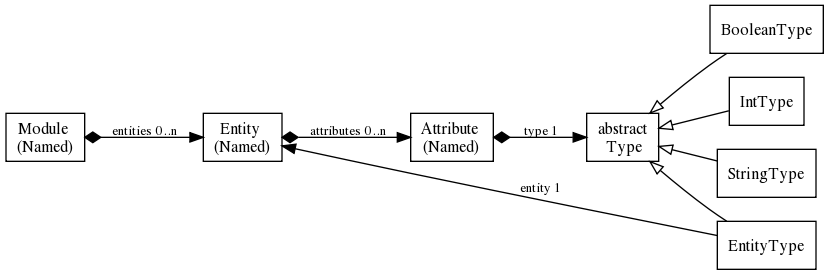
\includegraphics[scale=0.4]{figures/entities.png}
  \caption[labelInTOC]{The abstract syntax of the entities language. Entities
  have attributes, those have types and names. \ct{EntityType} extends 
  \ct{Type} and references \ct{Entity}. This "adapts" entities to types 
  (cf. the Adapter pattern). Concepts like \ct{EntityType} which have 
  exactly one reference are called smart references and are treated specially
  by the IDE in code completion. }
  \label{entities} 
\end{center}
\end{figure}

The following code shows the definition of the \ct{Entity} concept\footnote{This
is not the complete definition, concepts can have more characteristics. This is
simplified to show the essentials.}. \ct{Entity} extends \ct{BaseConcept}, the
root concept, similar to \ct{java.lang.Object} in Java. It implements the
\ct{INamedConcept} interface to inherit a \ct{name} field. It declares a list of
children of type \ct{Attribute} in the \ct{attributes} role. A concept may
also have references to other concepts (as opposed to children).


\begin{code}
concept Entity extends BaseConcept implements INamedConcept        
  is root:
    true
  properties:                                  
    << ... >>                                    
  children:                                     
    Attribute attributes 0..n specializes: <none>
  references:                                  
    << ... >>                                    
\end{code}                                               


Editors in MPS are based on cells. Cells are the smallest unit relevant for
projection. Defining an editor hence consists of arranging cells and defining
their content. Different cell types are available to compose editors.
\fig{editordefinition} explains the editor for \ct{Entity}. The editors for the
other concepts are defined similarly.



\begin{figure}[htp]
\begin{center}
  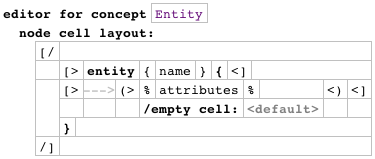
\includegraphics[scale=0.6]{figures/editordefinition.png}
  \caption[labelInTOC]{The editor for \ct{Entity}. The outermost cell is a
  vertical list. In the first line, we use a horizontal list that contains
  the "keyword" \ct{entity}, the value of the name property and an opening
  curly brace. In the second line we use indentation and a vertical arrangements
  of the contents of the \ct{attributes} collection. Finally, the third line
  contains the closing curly.}
  \label{editordefinition} 
\end{center}
\end{figure}

\phead{Type System} The MPS type system engine uses unification. Language
developers specify type equations and the unification engine tries to 
assign values to the type variables so that all equations are satisfied.
This is similar to what we know from math. Consider

\begin{code}
(1) 2 * x == 10
(2) x + x == 10
(3) x + y == 2 * x + 5
\end{code}


This set of equations can be solved by \verb#x := 5, y := 10#. The MPS type
system engine works the same way, but the domain is types instead of integers.
Type equations also don't just contain equations (:==:), but also equations
with subtyping and other relationships.

For the entities language, we specify two simple typing rules. The first one
specifies that the type of the primitives (\ct{int}, \ct{string}) is a
clone of themselves:

\begin{minipage}[t]{120mm}
\begin{code}
rule typeof_Type {                     
  applicable for concept = Type as type
  overrides false                      
  do {                                 
    typeof(type) :==: type.copy;       
  }                                    
}                                      
\end{code}
\end{minipage}

The only other typing rule is an equation that defines the type of the attribute
as a whole to be the type of the attribute's \ct{type} property, defined as
\verb#typeof(attribute) :==: typeof(attribute.type);#.


\phead{Generator} From entity models we generate Java Beans. Since Java is
available in MPS as the BaseLanguage, the generation is actually a
model-to-model transformation: from the entities model we generate a Java model.
MPS supports several kinds of transformations. The default case is the
template-based transformation which uses the concrete syntax of the target
language to specify model-to-model transformations. Alternatively, one can use
the node API to manually construct the target tree. Finally the 
textgen DSL is available to generate ASCII text (at the end of the
transformation chain). Throughout this paper we use the template based
approach.

Template-based generators in MPS consist of two main building blocks: mapping
configurations and templates. Mapping configurations define which elements are
processed with which templates. For the entities language, we need a \emph{root
mapping rule} and \emph{reduction rules}. Root mapping rules can be used to
create new top level artifacts from existing top level artifacts (they map
fragments to other fragments). In our case we generate a Java class from an
entity. Reduction rules are in-place transformations. Whenever the engine
encounters an instance of the specified source concept somewhere in a model
tree, it removes that source node and replace it with the result of the
associated template. In our case we have to reduce the various types (\ct{int},
\ct{string}, etc.) to their Java counterparts. \fig{entitiesmc} shows a part of
the mapping configuration for the entities language.


\begin{figure}[htp]
\begin{center}
  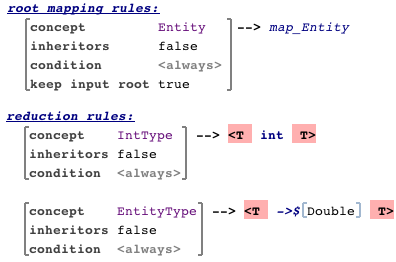
\includegraphics[scale=0.55]{figures/entitiesmc.png}
  \caption[labelInTOC]{The mapping configuration for the entities language. The
  root mapping rule for Entity specifies that instances of \ct{Entity} should
  be transformed with the \ct{map\_Entity} template. The reduction rules use
  inline templates. For example, the \ct{IntType} is replaced with the Java
  \ct{int} and the \ct{EntityRefType} is reduced to a reference to the class
  generated from the target entity. The arrow-dollar-symbol is a so-called
  reference macro. It contains code (not shown) that "rewires" the reference to
  \ct{Double} to a reference to the class generated from the target entity. }
  \label{entitiesmc} 
\end{center}
\end{figure}

MPS templates work differently from normal text generation templates such as for
example Xpand, Jet or StringTemplate, since they are actually model-to-model
transformations. Developers first write a structurally correct example model
using the target language. Then so called macros are used to change the example
model to reflect the input from which we generate. \fig{entitytemplate} shows
the \ct{map\_Entity} template. It generates a complete Java class --- notice the
complete structure of a Java class is present, because that is how BaseLanguage
defines the editor for a Java class. We then generate a field for each entity
\ct{Attribute}. To do this we first create a prototype field in the class
(\verb+private int aField;+). Then we use macros to "transform" this prototype
into an instance for each entity attribute. We first attach a \ct{LOOP} macro to
the whole field. It contains an expression \verb+node.attributes;+ where
\ct{node} refers to the input \ct{Entity}. This code is entered in the Inspector
window and is not shown in the screenshot. We then use a \ct{COPY\_SRC} macro to
transform the type. \ct{COPY\_SRC} copies the input node (the inspector
specifies the current attribute's type as the input here) and applies reduction
rules. So instances of the types defines as part of the entities language are
transformed into a Java type using the reduction rules defined in the mapping
configuration. Finally we use a property macro (the dollar sign) to change the
\ct{name} property of the field we generate from the dummy value \ct{aField} to
the name of the attribute we currently transform (once again via an expression
in the inspector).


\begin{figure}[htp]
\begin{center}
  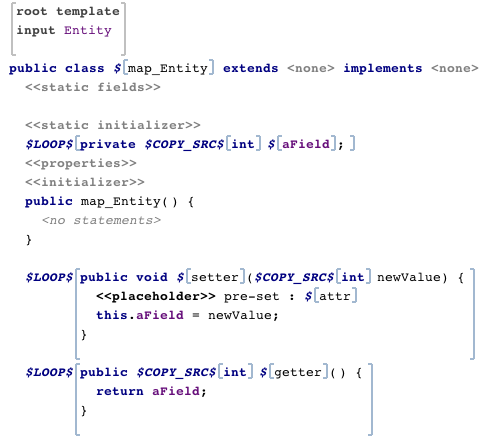
\includegraphics[scale=0.55]{figures/entitytemplate.png}
  \caption[labelInTOC]{The template for creating a Java class from an entity.
  The running text explains the details.}
  \label{entitytemplate} 
\end{center}
\end{figure}




\section{Implementing Language Extensions with MPS}
\label{extAndComp}


\subsection{Language Combination}

\phead{Structure and Syntax} We define a language uispec for defining user
interface forms based on the entities. \fig{uispec} shows the abstract syntax
and below is an example model. Note how the form is another, separate fragment.
It is a \emph{dependent} fragment, since it references elements from another
fragment (expressed in the entities language). Both fragments are
\emph{homogeneous} since they consist of sentences expressed in a single
language.

\begin{code}
form CompanyStructure                                                                                                                                  
  uses Department                                                                                                                                      
  uses Employee                                                                                                                                        
  field Name: textfield(30) -> Employee.name                                                                      
  field Role: combobox(Boss, TeamMember) -> Employee.role                                                                                              
  field Freelancer: checkbox -> Employee.freelancer
  field Office: textfield(20) -> Department.description                                                                                                
\end{code}

\begin{figure}[htp]
\begin{center}
  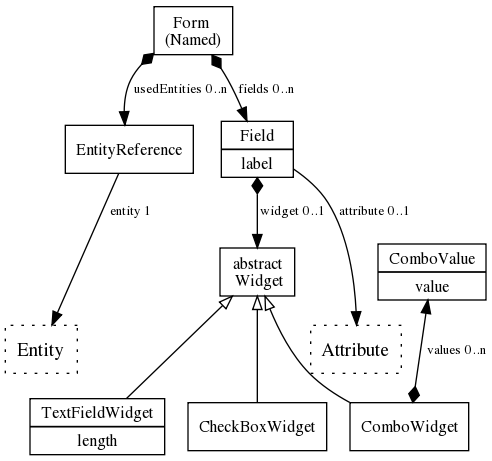
\includegraphics[scale=0.5]{figures/uispec.png}
  \caption[labelInTOC]{The abstract syntax of the uispec language. Dotted lines
  represent classes from another language (here: the entities language). A
  \ct{Form} contains \ct{EntityReference}s that connect to an entities model. A
  form also contains \ct{Field}s, each referring to an \ct{Attribute} from an
  \ct{Entity} and containing a \ct{Widget}.}
  \label{uispec} 
\end{center}
\end{figure}

The uispec language extends\footnote{MPS uses the term "extension" whenever the
definition of one language uses or referes to concepts defined in another
language. This is not necessarily an example of language extension as defined in
this paper.} the entities language. This means, that concepts from the entities
language can be used in the definition of language concepts in the uispec
language. A \ct{Form} owns a number of \ct{EntityReferences}, which in turn
reference the \ct{Entity} concept. Also, \ct{Field}s refer to the \ct{Attribute}
that shall be edited via the field. Here is the definition of the \ct{Field}
concept. It owns a \ct{Widget} and refers to an \ct{Attribute}.

 
\begin{code}
concept Field extends BaseConcept implements <none>               
  properties:                                 
    label : string                              
  children:                                   
    Widget widget 0..1 specializes: <none>      
  references:                                 
    Attribute attribute 0..1 specializes: <none>
\end{code}                                                                                            


\phead{Type System} There are limitations regarding which widget can be used
with which attribute type. This typing rule is defined in the uispec language
and references types from the entities language. The following is the code for
the type check. We use a non-typesystem rule to illustrate how constraints can
be written that do not use the inference engine introduced above.

\begin{code}
non type system rule checkTypes {                                                                                                                                                                                                                                                                                                                        
  applicable for concept = Field as field                                                                                                                                                                                                                                                                                                                
  overrides false                                                                                                                                                                                                                                                                                                                                        
  do {                                                                                                                                                                                                                                                                                                                                                   
    if (field.widget.isInstanceOf(CheckBoxWidget) 
         && !(field.attribute.type.isInstanceOf(BooleanType))) { 
      error "checkbox can only be used with booleans" -> field.widget; 
    } 
    if (field.widget.isInstanceOf(ComboWidget) 
         && !(field.attribute.type.isInstanceOf(StringType))) { 
      error "combobox can only be used with strings" -> field.widget; 
} } }
\end{code}


\phead{Generation} The defining characteristic of language combination is that
the two languages only reference each other, and the instance fragments are
dependent, but homogeneous. No syntactic integration is necessary in this case.
In this example, the generated code exhibits the same separation. From the form
definition, we generate a Java class that uses Java Swing to build the form. It
\emph{uses} the beans generated from the entities. The classes are instantiated,
and the setters are called. The generators are separate but they are
\emph{dependent}, they share information. Specifically, the forms generator
knows about the names of the generated entity classes, as well as the names of
the setters and getters. This is implemented by defining a couple of
behaviour methods on the \ct{Attribute} concept that are called from both
generators (the colon represents the node cast operator and binds tightly; the
code below casts the attribute's parent to \ct{Entity} and then accesses the
\ct{name} property).


\begin{code}
concept behavior Attribute {                                                 
  public string qname() {                                                    
    this.parent : Entity.name + "." + this.name;                             
  }                                                                          
  public string setterName() {                                               
    "set" + this.name.substring(0, 1).toUpperCase() + this.name.substring(1);
  }                                                                          
  public string getterName() {                                               
    "get" + this.name.substring(0, 1).toUpperCase() + this.name.substring(1);
  }                                                                          
}                                                                            
\end{code}


The original entities fragment is still \emph{sufficient} for the transformation
that generates the Java Bean. The form fragment is not sufficient for generating
the UI, it needs the entity fragment. This is not surprising since
\emph{dependent} fragments can never be sufficient for a transformation, the
transitive closure of all dependencies has to be made available.

\subsection{Language Extension}

We will revisit language extension later for more meaningful examples
of extension. For now, we extend the MPS base language with expression blocks
and placeholders. These concepts make writing generators \emph{that generate
base language code} much simpler. \fig{expressionBlock} shows an Example. We use
a screenshot instead of text because we use non-textual notations (the big
brackets) and color. 


\phead{Structure and Syntax} An expression block is a block that can be used
where an \ct{Expression} is expected \cite{BravenboerVVV05}. The block can
contain any number of statements; \ct{yield} can be used to "return values" from
within the block. So, in some sense, an expression block is an "inlined method",
or a closure that is defined and called directly. The optional name property of
an expression block is then used as the method name. The generator of the
expression block transforms it into just this structure:


\begin{code}
okButton.addActionListener(new ActionListener() {
  public void actionPerformed(ActionEvent p0) {
    Employee aEmployee = new Employee();
    aEmployee.setName(retrieve_name(aEmployee, widget0));
  }
  public String retrieve_name(Employee aEmployee, JComponent widget0) {
    String newValue = ((JTextField) widget0).getText();
    return newValue;
  }
}
\end{code}

\begin{figure}[htp]
\begin{center}
  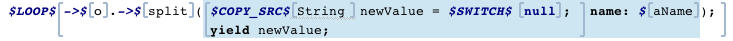
\includegraphics[scale=0.6]{figures/expressionBlock.png}
  \caption[labelInTOC]{Expression blocks (in blue) are basically anonymous
  inline methods. Upon transformation, a method is generated that contains the
  block content, and the expression block is replaced with a call to this
  method. Expression block are used mostly when implementing generators; this
  screenshot shows a generator that uses an expression block.}
  \label{expressionBlock} 
\end{center}
\end{figure}


The jetbrains.mps.baselanguage.exprblocks language extends MPS' BaseLanguage.
The expression block is used in places where the base language
expects an \ct{Expression}. This is why an \ct{BlockExpression} extends
\ct{Expression}. Consequently, fragments that use the exprblocks language, can
now use \ct{BlockExpression}s in addition to the concepts provided by the base
language. The fragments become \emph{heterogeneous}, because languaegs are
mixed.

\begin{code}
concept BlockExpression extends Expression implements INamedConcept
  children:                                     
    StatementList body 1 specializes: <none>      
\end{code}
          
\phead{Type System} The type of the \ct{yield} statement is the type of the
expression that is yielded, specified by 
\verb#typeof(yield) :==: typeof(yield.result);# (the type of /verb+yield 1;+
would be \ct{int}). Since the \ct{BlockExpression} is used as an expression, it
has to have a type as well. Since it is not explicitly specified, the type of
the \ct{BlockExpression} is the common super type of the types of all the
yields. The following typing rule computes this type:

\begin{code}
var resultType ; 
for (node<BlockExpressionYield> y : 
        blockExpr.descendants<concept = BlockExpressionYield>) { 
  resultType :==: typeof(y.result); 
} 
typeof(blockExpr) :==: resultType;
\end{code}
          
          
\phead{Generator} The generator for \ct{BlockExpression}s reduces the new 
concept to pure base
language: it performs assimilation. It transforms a heterogeneous fragment
(using BaseLanguage and exprblocks) to a homogeneous fragment (using only
BaseLanguage). The first step is the creation of the additional method 
for the block expression (\fig{expressionBlockGenerator1}).



% > 5.2 #Generator (Pg 12): AFAIK we have "extract method" instruction in
% > code generator. This was designed exactly for use case you are trying
% > to cover using weavings.



\begin{figure}[htp]
\begin{center}
  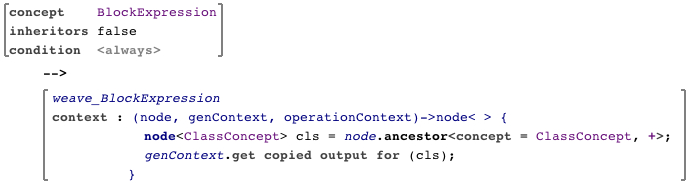
\includegraphics[scale=0.5]{figures/expressionBlockGenerator1.png}
  \caption[labelInTOC]{We use a weaving rule to create an additional method for
  this. A weaving rule processes an input element (\ct{BlockExpression}) by creating
  another node in a different place. The context function defines this
  other place. In this case, it simply gets the class in which we have defined
  the block expression.}
  \label{expressionBlockGenerator1} 
\end{center}
\end{figure}
 

The template shown in \fig{expressionBlockGenerator2} shows the creation of the
method. It assigns a mapping label to the created method. The mapping label
creates a a mapping between the \ct{BlockExpression} and the created method. We
will use this label to refer to this generated method when we generate the
method call that replaces the \ct{BlockExpression}
(\fig{expressionBlockGenerator3}).


\begin{figure}[htp] 
\begin{center}
  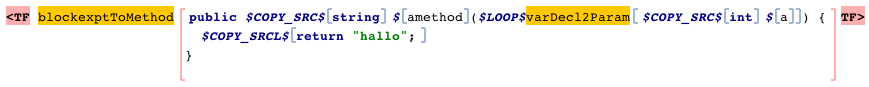
\includegraphics[scale=0.5]{figures/expressionBlockGenerator2.png}
  \caption[labelInTOC]{The generator creates a method from the block
  expression. It uses COPY\_SRC macros to replace the \ct{string} type with the
  computed return type of the block expression, inserts a computed name, adds a
  parameter for each referenced variable outside the block, and inserts all the
  statements from the block expression into the body of the method. The
  \ct{blockExprToMethod} mapping label is used later in the method call.}
  \label{expressionBlockGenerator2} 
\end{center}
\end{figure}



\begin{figure}[htp]
\begin{center}
  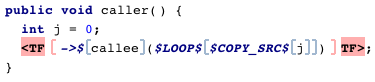
\includegraphics[scale=0.5]{figures/expressionBlockGenerator3.png}
  \caption[labelInTOC]{Here we generate the call to the previously generated
  method. We use the mapping label \ct{blockExprToMethod} to refer to the
  correct method (not shown; happens inside the ->\$ macro). We pass in the
  environment variables as actual arguments.}
  \label{expressionBlockGenerator3} 
\end{center}
\end{figure}

A second concept introduced by the exprblocks language is the
\ct{PlaceholderStatement}. It extends \ct{Statement} so it can be used
insider method bodies. It is used to mark locations at which subsequent
generators want to add additional code. These subsequent generators will use a
reduction rule to replace the placeholder with whatever they want to put at this
location. It is a means to building extensible generators, as we will see later.


\subsection{Language Reuse}

Language reuse covers the case where a language that has been developed
independent of the context in which it should be reused. The respective
fragments remain homogeneous. In this paper, we cover two alternative cases: the
first case addresses a persistence mapping language. The generated code is
separate of the code generated from the entities language. The second case
described a language for role-based access control. The generated code has to be
"woven into" the entities code to check permissions when setters are called.


\subsubsection{Separated Generated Code}

\phead{Structure and Syntax} relmapping is a reusable language for mapping
arbitrary data to relational tables. The relmapping language supports the
definition of relational table structures, but leaves the actual mapping to the
source data unspecified. As you adapt the language to a specific reuse context,
you have to specify this mapping. The following code shows the reusable part. A
database is defined that contains tables with columns. Columns have
(database-specific) data types.

\begin{code}
Database CompanyDB                          
  table Departments                         
    number id           
    char descr    
  table People                              
    number id                
    char name              
    char role              
    char isFreelancer
\end{code}

\fig{relmapping} shows the structure of the relmapping language. The abstract
concept \ct{ColumnMapper} serves as a hook: if we reuse this language
in a different context, we extend this hook by context-specific code. 

\begin{figure}[htp]
\begin{center}
  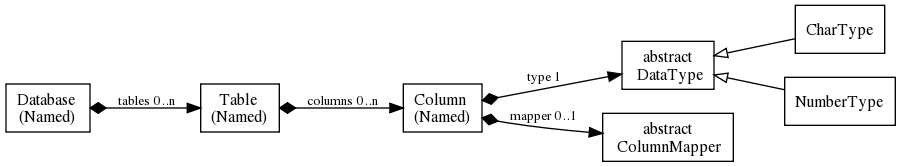
\includegraphics[scale=0.4]{figures/relmapping.png}
  \caption[labelInTOC]{A \ct{Database} contains \ct{Tables} which contain
  \ct{Columns}. A column has a name and a type. A column also has a
  \ct{ColumnMapper}. This is an abstract concept that determines where the
  column gets its data from. It is a hook intended to be specialized in
  sublanguages that are context-specific.}
  \label{relmapping} 
\end{center}
\end{figure}

 
The relmapping\_entities language extends relmapping and adapts it for reuse
with the entities language. To this end, it provides a subconcept
of \ct{ColumnMapper}, the \ct{AttributeColMapper}, which references an
\ct{Attribute} from the entities language as a means of expressing the mapping from the
attribute to the column. The column mapper is projected on the right of the
field definition, resulting in the following (heterogeneous) code fragment:


\begin{code}
Database CompanyDB                          
  table Departments                         
    number id <- Department.id              
    char descr <- Department.description    
  table People                              
    number id <- Employee.id                
    char name <- Employee.name              
    char role <- Employee.role              
    char isFreelancer <- Employee.freelancer
\end{code}


\phead{Type System} The type of a column is the type of its \ct{type} property.
In addition, the type of the column must also conform to the type of the column
mapper, so the concrete subtype must provide a type mapping as well. This
"typing hook" is implemented as an abstract behaviour method \ct{typeMappedToDB}
on the \ct{ColumnMapper}. It is acceptable from a dependency perspective to have
this typing hook, since relmapping is designed to be extensible. The typing
rules then look as follows:


\begin{code}
typeof(column) :==: typeof(column.type);
typeof(column.type) :==: typeof(column.mapper);
typeof(columnMapper) :==: columnMapper.typeMappedToDB();
\end{code}

The \ct{AttributeColMapping} concept from the relmapping\_entities implements
this method by mapping ints to numbers, and everything else to chars.

\begin{code}
public node<> typeMappedToDB() 
  overrides ColumnMapper.typeMappedToDB {                                                                          
  node<> attrType = this.attribute.type.type; 
  if (attrType.isInstanceOf(IntType)) { return new node<NumberType>(); } 
  return new node<CharType>();
}                                                                                                                                                  
\end{code}


\phead{Generator} The generated code is also separated into a reusable part (a
class generated by the generator of the relmapping language) and a
context-specific subclass of that class, generated by the relmapping\_entities
language. The generic base class contains code for creating the tables and for
storing data in those tables. It contains abstract methods that are used to
access the data to be stored in the columns. So the dependency structure of the
generated fragments, as well as the depdendencies of the respective generators,
resembles the dedpendency structure of the languages: the generated fragemnts
are dependent, and the generators are dependent as well (they share the name
(and implicitly the knowledge about the structure) of the class generated by the
reusable relmapping generator). A relmapping fragment (without the concrete
column mappers) is sufficient for generating the generic base class.


\begin{code}
public abstract class CompanyDBBaseAdapter {

  private void createTableDepartments() {
    // SQL to create the Departments table
  }

  private void createTablePeople() {
    // SQL to create the People table
  }

  public void storeDepartments(Object applicationData) {
    StringBuilder sql = new StringBuilder();
    sql.append("insert into" + "Departments" + "(");
    sql.append("" + "id");
    sql.append(", " + "descr");
    sql.append(") values (");
    sql.append("" + "\"" + getValueForDepartments_id(applicationData) + "\"");
    sql.append(", " + "\"" + getValueForDepartments_descr(applicationData) + "\"");
    sql.append(")");
  }

  public void storePeople(Object applicationData) {
    // like above
  }

  public abstract String getValueForDepartments_id(Object applicationData);

  public abstract String getValueForDepartments_descr(Object applicationData);

  // abstract getValue methods for the People table
}
\end{code}

The subclass, generated by the generator in the relmapping\_entities language
implements the methods defined by the generic superclass. The interface,
represented by the \ct{applicationData} object, has to be kept generic  so any
kind of user data can be passed in. Note how this class references the beans
generated from the entities. So the generator for entities and the generator
for relmapping\_entities are dependent, the information shared between the
two generator is the names of the classes generated from the entities.
The code generated from the relmapping language is designed to be extended by
code generated from a sublanguage (the abstract getValue methods). This is
acceptable, since the relmapping language itself is intended to be extended to
adapt it to a new reuse context.


\begin{code}
public class CompanyDBAdapter extends CompanyDBBaseAdapter {
  public String getValueForDepartments_id(Object applicationData) {
    Object[] arr = (Object[]) applicationData;
    Department o = (Department) arr[0];
    String val = o.getId() + "";
    return val;
  }
  public String getValueForDepartments_descr(Object applicationData) {
    Object[] arr = (Object[]) applicationData;
    Department o = (Department) arr[0];
    String val = o.getDescription() + "";
    return val;
  }
}
\end{code}
 


\subsubsection{Interwoven generated code}

\phead{Structure and Syntax} rbac is a language for specifying role-based access
control, to specify access permissions for the entities.

\begin{code}
RBAC                           
                               
users:                         
  user mv : Markus Voelter     
  user ag : Andreas Graf       
  user ke : Kurt Ebert         
                               
roles:                         
  role admin : ke              
  role consulting : ag, mv     
                               
permissions:                   
  admin, W : Department        
  consulting, R : Employee.name
\end{code}

The structure is shown in \fig{rbac}. Like relmapping, it provides a
hook, in this case, \ct{Resource}, to adapt it to context languages. The
sublanguge rbac\_entities provides two subconcepts of \ct{Resource}, namely
\ct{AttributeResource} to reference to an attribute, and \ct{EntityResource} to
refer to an \ct{Entity}, to define permissions for entities and their
attributes.


\begin{figure}[htp]
\begin{center}
  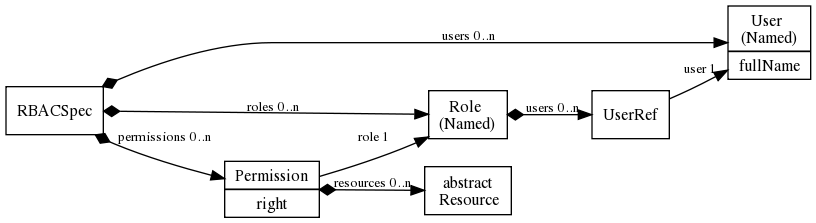
\includegraphics[scale=0.45]{figures/rbac.png}
  \caption[labelInTOC]{Language strucrure of the rbac language. An \ct{RBACSpec}
  contains \ct{Users}, \ct{Roles} and \ct{Permissions}. Users can be members 
  in several roles. A permission assigns a right to a \ct{Resource}.}
  \label{rbac}  
\end{center}
\end{figure}



\phead{Type System} No type system rules apply here.

\phead{Generator} What distinguishes this case from the relmapping case is that
the code generated from the rbac\_entities language is \emph{not} separated from
the code generated from the entities. Instead, inside the setters of the Java
beans, a permission check is required. 


\begin{code}
  public void setName(String newValue) {
    // check permissions (from rbac_entities) 
    if (new RbacSpecEntities().currentUserHasWritePermission("Employee.name")) {
      throw new RuntimeException("no permission");
    }
    this.name = newValue;
  }
\end{code}

The generated fragment is homogeneous (it is all Java code), but it is
\emph{multi-sourced}, since several generators contribute to the same fragment.
To implement this, several approaches are possible:


\begin{itemize}
  \item We could use AspectJ (\verb+http://www.eclipse.org/aspectj/+). This way,
  we could generate separate Java artifacts (all single-sourced) and then use the aspect weaver to "mix" them.
  However, we don't want to introduce AspectJ here, so we will not use this
  approach. 
  \item An interceptor (\verb+http://en.wikipedia.org/wiki/Interceptor_pattern+)
  framework could be added to the generated Java Beans, with the generated
  code contributing specific interceptors (effectively building a custom AOP solution). 
  We will not use this approach either, since it would require the addition of a 
  whole interceptor framework to the entities. This seems like overkill.
  \item We could "inject" additional code generation templates to the existing
  entities generator from the rbac\_entities generator. This would make the
  generators \emph{woven} as opposed to just dependent. Assuming this would work
  in MPS, this would be the most elegant solution. But it does not.
  \item We could define a hook in the generated Java beans code and then have
  the rbac\_entities generator contribute code to this hook. This is the
  appraoch we will use. The generators remain dependent, they have to agree on
  the way the hook works.
\end{itemize}








Notice that only the AspectJ solution can work without any preplanning from the
perspective of the entities language, because it avoids mixing the generated
code artifacts (it is handled "magically" by AspectJ). All other solutions
require the original entities generator to "expect" certain extensions.

In our case, we have modified the original generator in the entities language to
contain a \ct{PlaceholderStatement} (\fig{placeholder}). In every setter, the
placeholder acts as a hook at which subsequent generators can add statements.
While we have to preplan \emph{that} we want to extend the generator in this
place, we don't have to predefine \emph{how}. The placeholder contains a
key into the session object that points to the currently processed attribute.
This way, the subsequent generator can know from which attribute the method with
the placeholder in it was generated.


\begin{figure}[htp] 
\begin{center}
  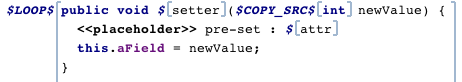
\includegraphics[scale=0.55]{figures/placeholder.png}
  \caption[labelInTOC]{This generator fragment creates a setter method for each
  attribute of an entity. The LOOP iterates over all attributes. The \$ macro
  computes the name of the method, and the COPY\_SRC macro on the argument type
  computes the type. The placeholder is used later to insert the
  permission check.}
  \label{placeholder}  
\end{center}
\end{figure}

The rbac\_entities generator contains a reduction rule for
\ct{PlaceholderStatement}s. So when it encounters a placeholder (that has been
put there by the entities generator) it removes it and inserts the code that
checks for the permission (\fig{placeholderreduction}). To make this work we
have to make sure that this generator runs \emph{after} the entities generator
(since the entities generator has to create the placeholder) and \emph{before}
the BaseLanguage generator (which transforms BaseLanguage code into Java text
for compilation). We use generator priorities, i.e. a partial ordering, to
achieve this.


\begin{figure}[htp] 
\begin{center}
  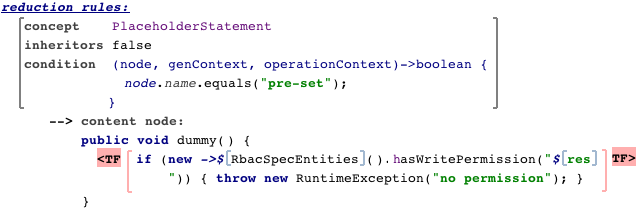
\includegraphics[scale=0.50]{figures/placeholderreduction.png}
  \caption[labelInTOC]{This reduction rule replaces \ct{PlaceholderStatement}s
  with a permission check. Using the condition, we only match those
  placeholders whose identifier is \ct{pre-set} (notice how we have defined
  this identifier in \fig{placeholder}). The inserted code queries another
  generated class that contains the actual permission check. A runtime
  exception is thrown if the check fails.}
  \label{placeholderreduction}  
\end{center}
\end{figure}


\subsection{Language Embedding}

\phead{Structure and Syntax} uispec\_validation extends uispec, it is a
sublanguage of the validation language. It supports writing code such as the
following in the UI form specifications. Writing the expressions is supported by
embedding a reusable expressions language. \fig{uival} shows the structure. To
be able to use the expressions, the user has to use a \ct{ValidatedField}
instead of a \ct{Field}. \ct{ValidatedField} is also defined in
uispec\_validation and is a subconcept of \ct{Field}.


\begin{code}
form CompanyStructure                                                                                                                                  
  uses Department                                                                                                                                      
  uses Employee                                                                                                                                        
                                                                                                                                                       
  field Name: textfield(30) -> Employee.name validate lengthOf(Employee.name) < 30                                                                     
  field Role: combobox(Boss, TeamMember) -> Employee.role                                                                                              
  field Freelancer: checkbox -> Employee.freelancer 
        validate if (isSet(Employee.worksAt)) Employee.freelancer == true else
                    Employee.freelancer == false 
  field Office: textfield(20) -> Department.description                                                                                                
\end{code}

\begin{figure}[htp]
\begin{center}
  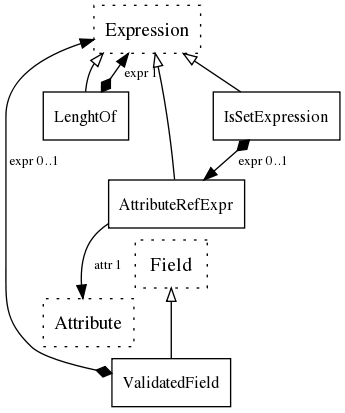
\includegraphics[scale=0.50]{figures/uival.png}
  \caption[labelInTOC]{The uispec\_validation language defines a subtype of
  \ct{uispec.Field} that contains an \ct{Expression} from a reusable expression
  language. The language also defines a couple of additional expressions,
  specifically the \ct{AttributeRefExpr}, which can be used to refer to
  attributes of entities.}
  \label{uival}  
\end{center}
\end{figure}

To support the migration of existing models that use \ct{Field} instances, we
provide an intention: the user can press Alt-Enter on a \ct{Field} and select
"Make Validated Field". This transforms an existing \ct{Field} into a
\ct{ValidatedField}, so that validation expressions can be entered. The core of
the intention is the following script, which performs the actual transformation:

\begin{code}
execute(editorContext, node)->void { 
    node<ValidatedField> vf = new node<ValidatedField>(); 
    vf.widget = node.widget; 
    vf.attribute = node.attribute; 
    vf.label = node.label; 
    node.replace with(vf); 
}
\end{code}


The uispec\_validation language extends the uispec language. We also extend the
existing, reusable expressions language, so we can use \ct{Expressions} in the
definition of our language. \ct{ValidatedField} has a property \ct{expr} that
contains the actual expression. As a consequence of polymorphism, we can use any
existing subconcept of \ct{Expression} here. So without doing anything else, we
could write \verb#20 + 40 > 10#, since integer literals and the plus operator
are defined as part of the composed expressions language. However, to write
anything useful, we have to be able to reference entity attributes from within
expressions. To achieve this, we create the \ct{AttributeRefExpr} as shown in
\fig{uival}. We also create \ct{LenghtOf} and \ct{IsSetExpression} as further
examples of how to adapt an embedded language to its new context ---
i.e. the uispec and entities languages.


The \ct{AttributeRefExpr} may only reference those attributes of those
entities that used in the form within which we define the validation expression.
The following is the code for the search scope:

\begin{code}
(model, scope, referenceNode, linkTarget, enclosingNode)
                             ->join(ISearchScope | sequence<node< >>) { 
  nlist<Attribute> res = new nlist<Attribute>; 
  node<Form> form = enclosingNode.ancestor<concept = Form, +>; 
  for (node<EntityReference> er : form.usedEntities) { 
    res.addAll(er.entity.attributes); 
  } 
  res; 
}
\end{code}

Notice that the actual syntactic embedding of the expressions in the
uispec\_validation language is no problem at all as a consequence of how
projectional editors work. We simply define \ct{Expression} to be a child of the
\ct{ValidatedField}. 


\phead{Type System} The general challenge here is that primitive types such as
\ct{int} and \ct{string} are defined in the entities language and in the
reusable expression language. Although they have the same names, they are not
the same types. So the two sets of types must be mapped. Here are a couple of
examples. The type of the \ct{IsSetExpression} is by definition
\ct{expressions.BooleanType}. The type of the \ct{LengthOf}, which takes an
\ct{AttrRefExpression} as its argument, is \ct{expressions.IntType}.
The type of an attribute reference is the type of the attribute's \ct{type} property, as in
\verb#typeof(are) :==: typeof(are.attr.type);#. However, consider now the
following code:

\begin{code}
  field Freelancer: checkbox -> Employee.freelancer 
        validate if (isSet(Employee.worksAt)) Employee.freelancer == true else
                    Employee.freelancer == false 
\end{code}

This code states that if the \ct{worksAt} attribute of an employee is set, then
its \ct{freelancer} attribute must be \ct{true} else it must be \ct{false}. It
uses the equals operator from the expressions language. However, that operator
expects two \ct{expressions.BooleanType} arguments, but the type of the
\ct{Employee.freelancer} is \ct{entities.BooleanType}. In effect, we have to
override the typing rules for the expressions languages's equals operator. Here
is how we do it, using \ct{Equals} as an example.

In the expressions language, we define so-called overloaded operation rules. We
specify the resulting type for an \ct{EqualsExpression} depending on its argument types.
Here is the code in the expressions language that defines the resulting type to
be \ct{boolean} if the two arguments are \ct{Equallable}:

\begin{code}
operation concepts: EqualsExpression                                                     
  left operand type: new node<Equallable>() 
  right operand type: new node<Equallable>() 
operation type:                                                                          
  (operation, leftOperandType, rightOperandType)->node< > { 
    <boolean>; 
  }               
\end{code}

In addition to this code, we have to specify that \ct{expressions.BooleanType}
is a subtype of \ct{Equallable}, so this rule applies if we use equals with two 
\ct{expressions.BooleanType} arguments. We have to tie this overloaded operation
specification into a regular type inference rule.

\begin{code}
rule typeof_BinaryExpression {                                                                                                                                                                                                                                                                                                                                                                                                                                                   
  applicable for concept = BinaryExpression as binaryExpression                                                                                                                                                                                                                                                                                                                                                                                                                  
  overrides false                                                                                                                                                                                                                                                                                                                                                                                                                                                                
                                                                                                                                                                                                                                                                                                                                                                                                                                                                                 
  do {                                                                                                                                                                                                                                                                                                                                                                                                                                                                           
    when concrete (typeof(binaryExpression.left) as left) { 
      when concrete (typeof(binaryExpression.right) as right) { 
        node<> opType = operation type( binaryExpression , left , right ); 
          if (opType != null) { 
            typeof(binaryExpression) :==: opType; 
          } else { 
            error "operator " + binaryExpression.concept.name + 
                  " cannot be applied to these operand types " + 
                  left.concept.name + "/" + right.concept.name 
               -> binaryExpression; } 
}  }  }  } 
\end{code}

To override these typing rules to work with \ct{entities.BooleanType}, we simply
provider another overloaded operation specification in the uispec\_validation
language:

\begin{code}
operation concepts: EqualsExpression                                       
  one operand type: <boolean> // this is the entities.BooleanType!     
operation type:                                                            
  (operation, leftOperandType, rightOperandType)->node< > { 
    <boolean>;  // this is the expressions.BooleanType 
  } 
\end{code}


\phead{Generator} The generator has to create BaseLanguage code, which is then
subsequently transformed into Java Text. To deal with the transformation of the
expressions language, we can do one of two things:

% > - create own text gen (just like it's done for BaseLanguage
% > constructions). This way of generating code looks more straight
% > forward then "wrapping expressions into some kind of
% > TextHolderStatement".
% > - reduce expressions to a BaseLanguage constructions (the second
% > choice proposed in paper).
% >
% > I think TextHolderStatement can be mentioned here as an option, but
% > MPS textgen looks like a native way to produce textual output from the
% > model.


\begin{itemize}
  \item Either we can use the expression's language existing to-text generator
  and wrap the expressions in some kind of \ct{TextHolderStatement}. Remember
  that we cannot simply embed text in BaseLanguage, since that would not work
  structurally. A wrapper is necessary.
  \item Alternatively, we can write a (reusable) transformation from expressions
  code to BaseLanguage code; these rules would get used as part of the
  transformation of uispec and uispec\_validation code to BaseLanguage.
\end{itemize}

Since many DSLs will map code to BaseLangauge, it is worth the effort to
write a reusable generator from uispec\_validation expressions to BaseLanguage
expressions. We choose this second alternative. The generated Java code is
multi-sourced, since it is generated by two independent code generators.


Expression constructs from the reusable expr language and those of BaseLanguage
are almost identical, so this generator is trivial. We create a new language
project de.voelter.mps.expressions.blgen and add reduction rules.
\fig{expr2blgen} shows some of these reduction rules.


\begin{figure}[htp]
\begin{center}
  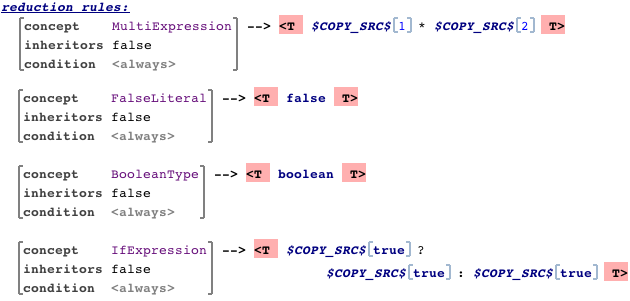
\includegraphics[scale=0.50]{figures/expr2blgen.png}
  \caption[labelInTOC]{A number of reduction rules that map the reusable
  expression language to BaseLanguage (Java). Since the languages are very
  similar, the mapping is trivial. For example, a \ct{PlusExpression} is mapped
  to a + in Java, the left and right arguments are reduced recursively through
  the COPY\_SRC macro.}
  \label{expr2blgen}  
\end{center}
\end{figure}

In addition to these, we also need reduction rules for those new expressions
that we have added specifically in the uispec\_validation language
(\ct{AttrRefExpression, isSetExpression, LengthOf}). Those are defined in
uispec\_validation. As an example, \fig{reductionAttributeRef} shows the rule
for handling the \ct{AttrRefExpression}. The validation code itself is
"injected" into the UI form via the same placeholder reduction as in the case of
the rbac\_entities language.


\begin{figure}[htp]
\begin{center}
  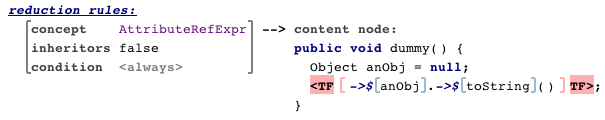
\includegraphics[scale=0.50]{figures/reductionAttributeRef.png}
  \caption[labelInTOC]{References to entity attributes are mapped to a call to
  their getter method. The tempalte fragment (inside the TF) uses two reference
  macros (->\$) to "rewire" the object reference to the Java bean instance, and
  the \ct{toString} method call to a call to the getter.}
  \label{reductionAttributeRef}  
\end{center}
\end{figure}

Language extension can also be used to prohibit the use of certain concepts of
the base language in the sublanguage, at least in certain contexts. As a simple
(but admittedly relatively useless) example, we restrict the use of certain
operators provided by the reusable expression language insider validation rules
in uispec\_validation. This can be achieved by implementing a 
\ct{can be ancestor} constraint on \ct{ValidatedField}.

\begin{code}
can be ancestor:
  (operationContext, scope, node, childConcept)->boolean { 
    return !(childConcept == concept/GreateEqualsExpression/ || 
             childConcept == concept/LessEqualsExpression/); 
  }
\end{code}


\subsection{Language Annotations}

\phead{Structure and Syntax} Since in a projectional editor the visual
representation of a program is not necessarily the complete information in the
program, and since the program's persistence format is not the concrete
syntax, it is possible to store additional data in a program, and show it
optionally. The mechanism MPS uses for this is called annotations.
Using this approach, we can store the mapping from entity attributes to database
columns directly in the entity, resulting in the following code:


\begin{code}
module company                                 
  entity Employee {                            
    id : int -> People.id                      
    name : string -> People.name               
    role : string -> People.role               
    worksAt : Department -> People.departmentID        
    freelancer : boolean -> People.isFreelancer
  }                                            
                                            
  entity Department {                          
    id : int -> Departments.id                 
    description : string -> Departments.descr  
  }                                            
\end{code}

This is a heterogeneous fragment, consisting of code from the entities, as well
as the annotations. From a concrete syntax perspective, the column mapping is
"embedded" in the entity description. In the underlying persistent data
structure, the information is also actually stored in the entity model. However,
the definition of the entities language does not know that this additional
information is stored and projected "inside" entities! No modification to the
entities language is necessary whatsoever. Instead we define an additional
language relmapping\_annotations which extends the entities language as well as
the relmapping language. In this language we define a so-called annotation link:


\begin{code}
annotation link declaration colMapping
    stereotype node                   
    cardinality 1                     
    source Attribute                  
    target AttrToColMapping           
\end{code}

This must be read as follows: we create an annotation for \ct{Attribute} which
can point to one instance of \ct{AttrToColMapping}. \ct{AttrToColMapping} is
simply another concept that has one reference that points to a \ct{Column}:

\begin{code}
concept AttrToColMapping extends BaseConcept implements <none>  
  references:                               
    Column column 1 specializes: <none>       
\end{code}                                            

Structurally, an annotation is a child of the node it is annotated to. So the
\ct{Attribute} has a new child of type \ct{AttrToColMapping}, and the reference
that contains the child is called \ct{@colMapping}. However, in the editor the
relationship is reversed. The editor for \ct{AttrToColMapping} wraps the editor
for \ct{Attribute}, as \fig{annotationeditor} shows. The annotation is added via
an intention ("quick fix" via Alt-Enter).


\begin{figure}[htp]
\begin{center}
  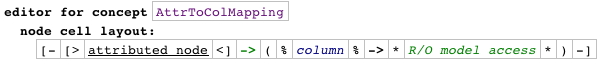
\includegraphics[scale=0.55]{figures/annotationeditor.png}
  \caption[labelInTOC]{The editor for the \ct{AttrToColMapping} embeds the
  editor of the concept it is annotated to (using the \ct{attributed node}
  cell). It then projects the reference to the referenced column.}
  \label{annotationeditor}  
\end{center}
\end{figure}


Note that it is also possible to define the annotation source to be
\ct{BaseConcept}, which means the annotation can be attached to any node. The
language that contains the annotation then has no dependency to any other
language. This is useful for generic "metadata" such as documentation,
requirements traces or presence conditions in product line engineering. We have
described this in \cite{VoelterVisser2011} and \cite{Voelter2010}.

\phead{Type System} The same typing rules are necessary as in the
relmapping\_entities language described above. They reside in
relmapping\_annotations.

\phead{Generator} The generator is also broadly similar to the above example
with relmapping\_entities. It takes the entities model as the input, and then
uses the column mappings in the annotations to create the entity-to-database
mapping code.

\vspace{10pt}
The annotations introduced above were typed to be specific to certain target
concepts (\ct{EntityAttribute} in this case). A particularly interesting use of
of annotations includes those that can be annotated to \emph{any} language
concept (formally targetting \ct{BaseConcept}). In this case, there is no
dependency between the language that contains the annotation and the language
that is annotated. This is very useful for "meta data", as well as anything that
can be processed generically. 

An example of the first case is traceability links (\fig{requirementstrace}).
This annotation can be annotated to any language concept and adds pointers
(trace links) to requirements. As a consequence of the projectional approach,
the program can be shown with or without the annotations, controlled by a global
switch.

\begin{figure}[htp]
\begin{center}
  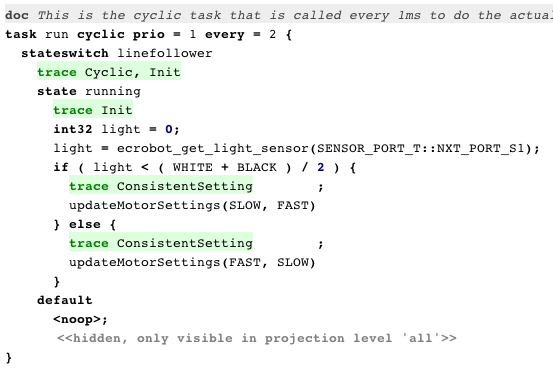
\includegraphics[scale=0.50]{figures/requirementstrace.png}
  \caption[labelInTOC]{Requirements traces can be annotated to any arbitrary
  program element. The annotation is targetted to \ct{BaseConcept}, which means
  there is no explicit dependency any specific language.}
  \label{requirementstrace} 
\end{center}
\end{figure}

An example of the second case is product line variability annotations
(\fig{featuredependencies}). Boolean expressions over configuration switches can
be annotated to any model element. Such an annotation means that the respective
element is only in the program variant, if the boolean expression is true for
the given setting of configuration switches. The generic transformation simply
removes all elements whose annotation evaluates to false. The expressions can
also be evaluated as part of the projection, showing the code for a given
variant. The code is of course still editable. Details on this approach can be
found in \cite{Voelter2010} and \cite{VoelterVisser2011}.

\begin{figure}[htp]
\begin{center}
  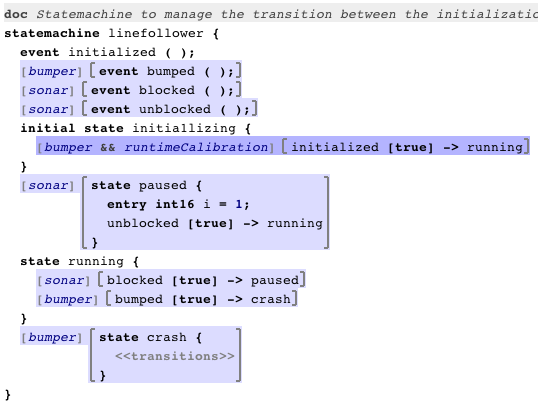
\includegraphics[scale=0.50]{figures/featuredependencies.png}
  \caption[labelInTOC]{Feature dependency annotations are boolean expresssions
  over configuration switches that determine whether the annotated program
  element is part of a program variant. The transformation removes all those
  elements for which the annotation evaluates to false.}
  \label{featuredependencies}  
\end{center}
\end{figure}

\begin{figure}[htp]
\begin{center}
  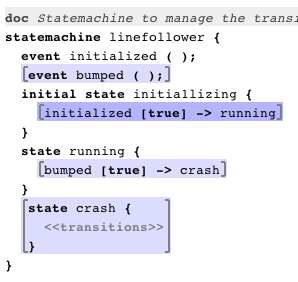
\includegraphics[scale=0.50]{figures/featureCutDown.png}
  \caption[labelInTOC]{This is the statemachine from \fig{featuredependencies},
  customized to the variant where only the \emph{bumper} switch is turned on.
  The \emph{bumper}-specific parts are highlighted.}
  \label{featureCutDown}  
\end{center}
\end{figure}








\section{Evaluation}
\label{Eval}

The examples above show that meaningful LME\&C is possible with MPS.
Specifically, reuse and embedding of languages is possible. The challenge
of grammar composition is not an issue in MPS at all, since no grammars and
parsers are used. The fact that we hardly ever discuss syntactic issues in the
above discussions is proof of this. 

However, extensibility regarding the other aspects is a bit less well
structured:

\begin{itemize}
  \item In case of generators, language designers have to specify a partial
  ordering of mapping configurations using priorities. It is not easily possible
  to "override" an existing generator, but generators can run \emph{before}
  existing ones. Generator extension is not possible directly, this is why we
  use the placeholders that are put in by earlier generators to be reduced by
  later ones.
  \item The concrete syntax for elements of the base language cannot be
  overridden in the sublanguage, although this is supposed to change.
  \item Overriding of scopes is not possible; a workaround exists by factoring
  the code into a virtual method (and calling it from the scope).
  \item Typing rules cannot be overridden unless an overloaded operation rules
  container is used in the original language.
\end{itemize}

In my opinion, a consistent approach for extending and overriding aspects of the
original language is missing. I suggest an approach called \emph{Generic
Outside, Specific Inside}. It is basically a variant of component-based design
(\verb+http://en.wikipedia.org/wiki/CBD+). All
language aspects use components as the core structural building block.
Components have types. The type of the component determines the kinds of facets
it has. A facet is a kind of interface that exposes the (externally visible)
ingredients of the component. The kinds of ingredients depend on the component
type: a component of type \emph{structure} exposes language concepts. A
component of type \emph{editor} exposes editors, type \emph{type system} exposes
type system rules, and so on. Each component type would use a different DSL for
implementation. Here is the important point: a component (in a sublanguage) can
specify an \emph{advises} relationship to another component (from a super
language). Then each of the facets can determine which facets from the advised
component it wants to \emph{preempt}, \emph{enhance} or \emph{override}.
\fig{gosi} shows the meta model of the approach.


\begin{figure}[htp]
\begin{center}
  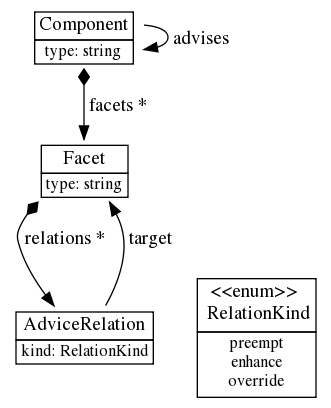
\includegraphics[scale=0.45]{figures/gosi.png}
  \caption[labelInTOC]{Components contain facets. Facets come in different
  kinds and the component type determines which facets types are available. The
  facets export the component's contribution to a language. Facets can
  declare relations to other facets (preempt, enhance, override) as a generic
  way to change the contributions exported by components of a base language.}
  \label{gosi}  
\end{center}
\end{figure}

This approach would provide the same way of packaging behavior for all language
aspects, as well as a single, consistent way of changing that behavior in a
sublanguage:

\begin{itemize}
  \item \emph{preemption} means that the respective behavior is contributed
  before the the behavior from the base language. A generator may use this to reduce a
  construct before the original generator gets a chance to reduce the construct. 
  \item \emph{enhancement} means that the sublanguage component is executed
  after the advised component from the base language. Notice that for declarative aspects
  where ordering is irrelevant, preempt and enhance are exchangable.
  \item \emph{overriding} means that the original facet is completely
  shadowed by the new one. This could be used for example to define a new editor for an existing
  construct.
\end{itemize}

To control the granularity at which preemption, enhancement or overriding is
performed, the base language designed would have to group his structures or
behaviors into suitably cut facets. This amount of preplanning is acceptable: it
is just as in OO programming, where behavior that should be overridable has to
be packaged into its own method.
  
The approach could be taken further. Components could be marked as
\emph{abstract}, and define a set of parameters for which values need to be
provided by non-abstract subcomponents. A language is abstract as long as it has
at least one abstract component, for which no concrete subcomponent is provided.
Component parameters could even be usable in structure definitions, for example
as the base concept; this would make a language parametrizable regarding the
base language it extends from.

In essence, the suggested approach is a bit like object orientation (components
== classes, facets == methods), with a rich advise framework (as in AOP).
Component parameters typed to language concepts are similar to generics. Using
this approach, a powerful and consistent approach to language extensibility
would be available.

\section{Summary}
\label{Summary}

MPS is powerful environment for language engineering. While not all of its
features are unique (see \sect{Related}), the combination of flexible
composition and the notational freedom as a consequence of the projectional
approach is certainly convincing. I also want to emphasize that the tool also
scales to realistic program sizes, the editor is very usable, and it integrates
well with existing VCS (diff and merge is provided on the level of the concrete
syntax). At the very minimum, the tool is a perfect environment for language
experimentation in the context of academic and industrial research.

The major drawback of MPS is its non-trivial learning curve. Because it works so
differently than traditional language engineering environments, and because it
addresses so many aspects of languages (incl. type systems, data flow and
refactorings) mastering the tools takes a significant investment in terms of
time. I hope that in the future this investment will be reduced by better
documentation and better defaults, to keep simple things simple and complex
things tractable. First ideas exist on how this could be done.


 


%\begin{acknowledgements}
%If you'd like to thank anyone, place your comments here
%and remove the percent signs.
%\end{acknowledgements}

% BibTeX users please use one of
%\bibliographystyle{spbasic}      % basic style, author-year citations
%\bibliographystyle{spmpsci}      % mathematics and physical sciences
%\bibliographystyle{spphys}       % APS-like style for physics
%\bibliography{}   % name your BibTeX data base

\bibliographystyle{abbrv}
\bibliography{fromResearchr}



\end{document}
% end of file template.tex

